%%%%%%%%%%%%%%%%%%%%%%%%%%%%%%%%%%%%%%%%%%%%%%%%%%%%%%%%%%%%%%%%%%%
%                                                                 %
%  GEANT manual in LaTeX form                              %
%                                                                 %
%  Michel Goossens (for translation into LaTeX)                   %
%  Version 1.00                                                   %
%  Last Mod. Jan 24 1991  1300   MG + IB                          %
%                                                                 %
%%%%%%%%%%%%%%%%%%%%%%%%%%%%%%%%%%%%%%%%%%%%%%%%%%%%%%%%%%%%%%%%%%%
\Origin{R.Brun, M.Maire}
\Revision{F.Carminati, S.Giani, L.Urb\'{a}n}
\Submitted{01.10.84}    \Revised{16.12.93}
\Version{Geant 3.16}    \Routid{TRAK200}
\Makehead{The tracking routines block diagrams}
 
\begin{figure}[hbt]
     \centering
     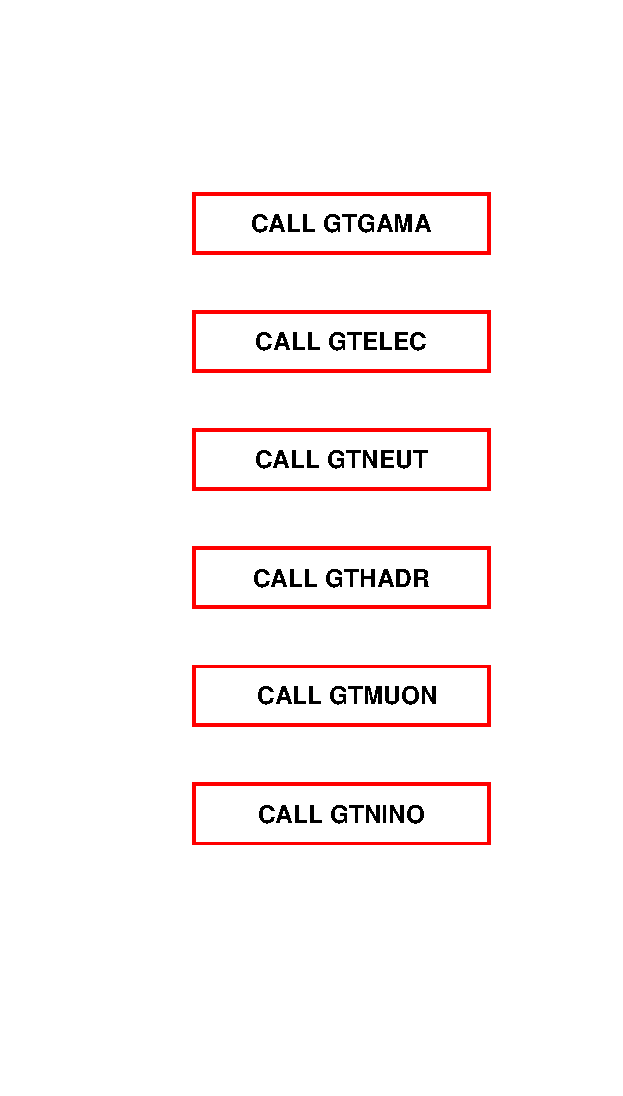
\epsfig{file=eps/trak200-1.eps,width=10cm}
     \caption{The traking routines}
     \label{fg:trak200-1}
\end{figure}

\begin{figure}[hbt]
     \centering
     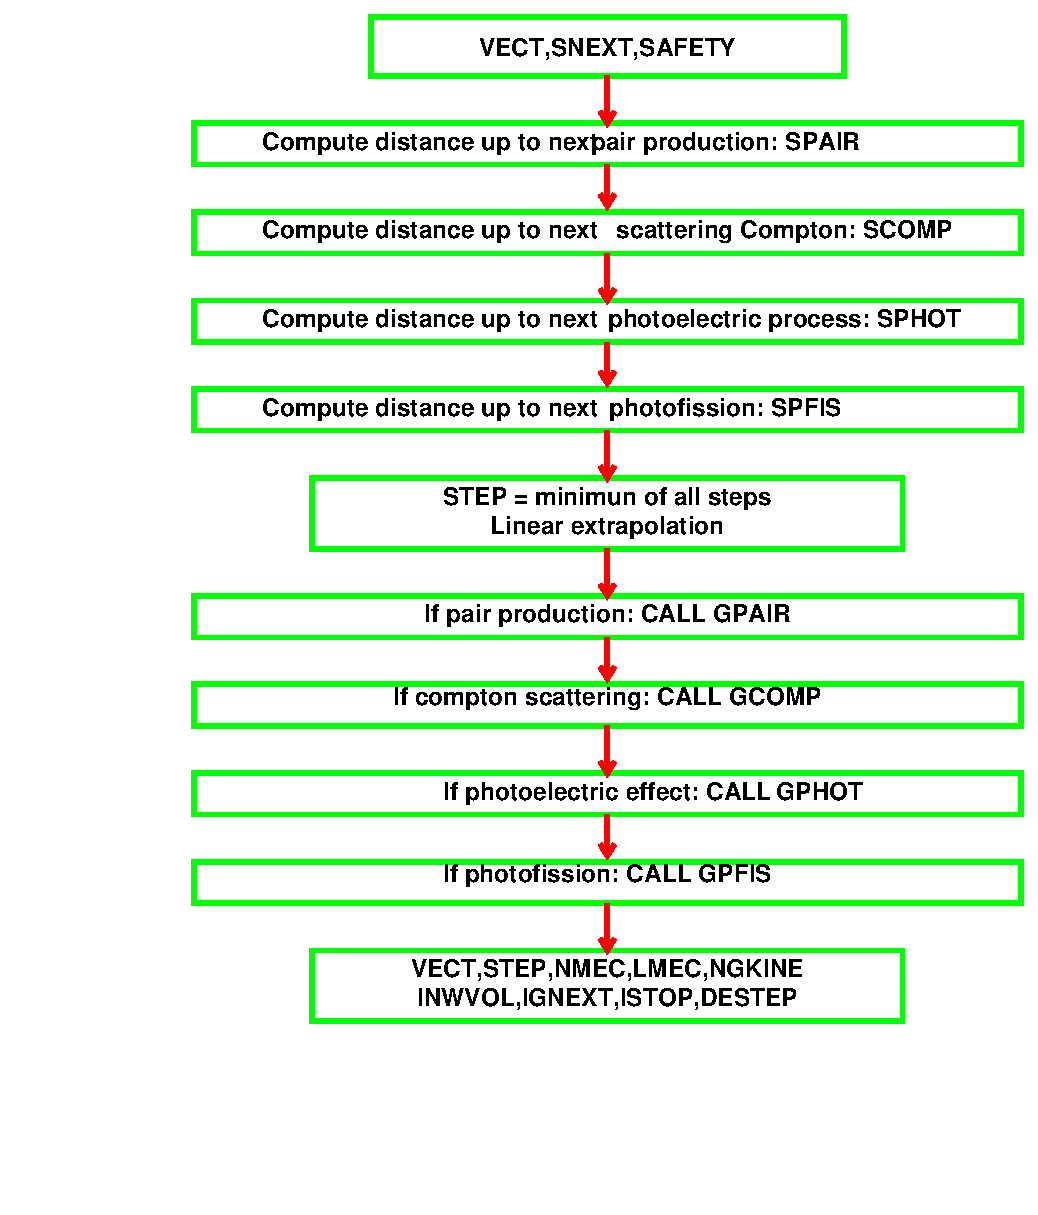
\epsfig{file=eps/trak200-2.eps,width=14cm}
     \caption{{\tt GTGAMA} block diagram}
     \label{fg:trak200-2}
\end{figure}

\begin{figure}[hbt]
     \centering
     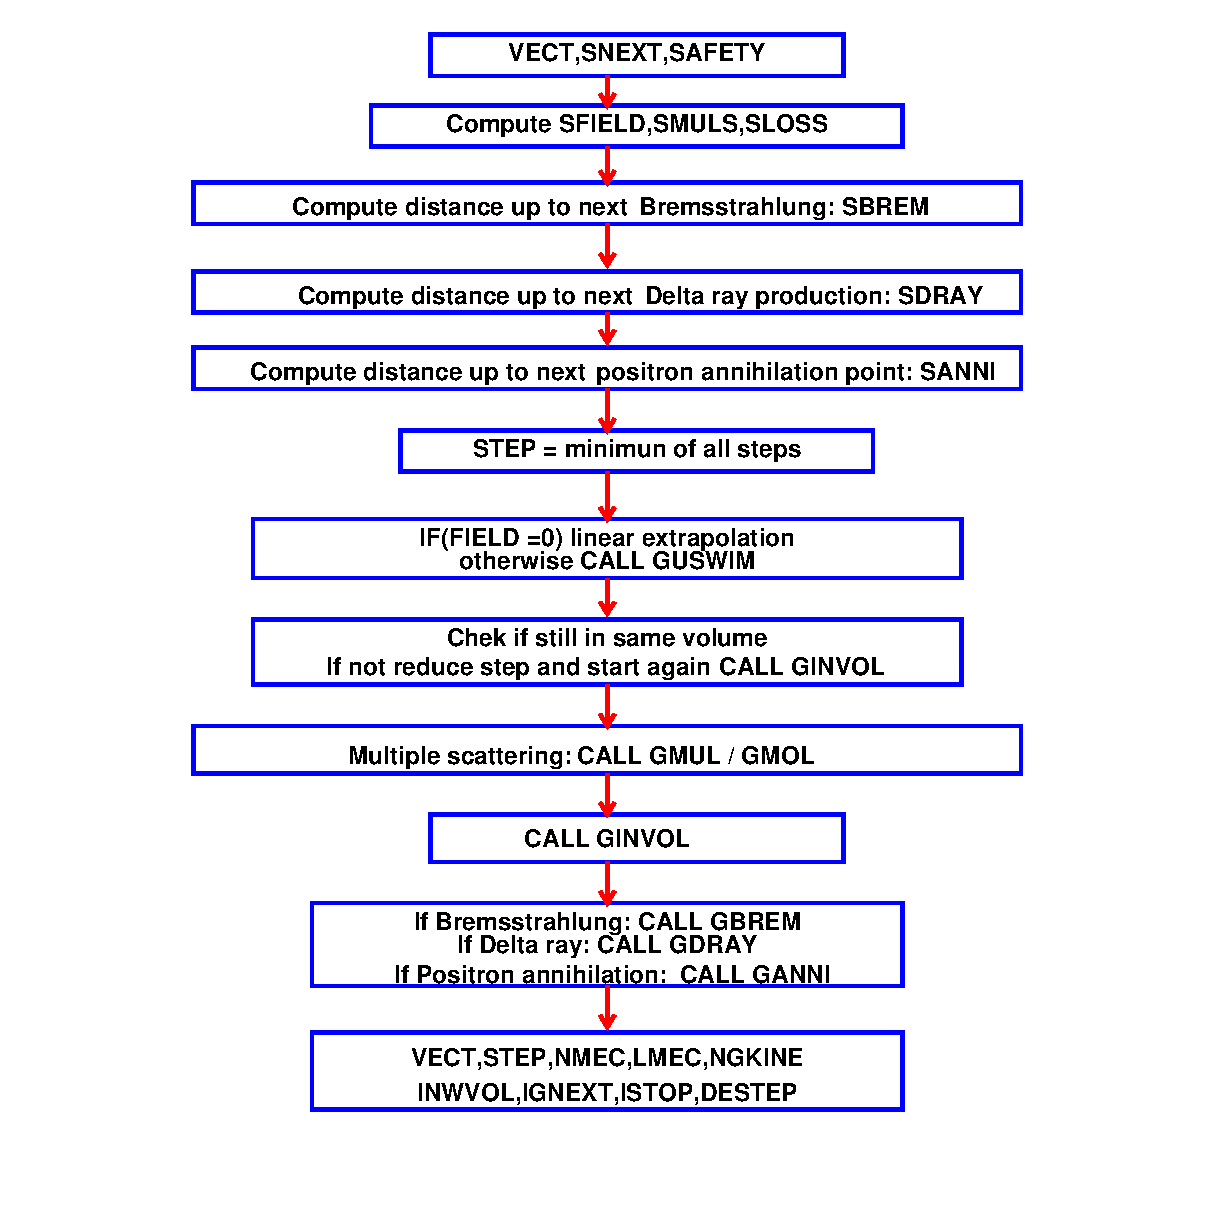
\epsfig{file=eps/trak200-3.eps,width=14cm}
     \caption{{\tt GTELEC} block diagram}
     \label{fg:trak200-3}
\end{figure}

\begin{figure}[hbt]
     \centering
     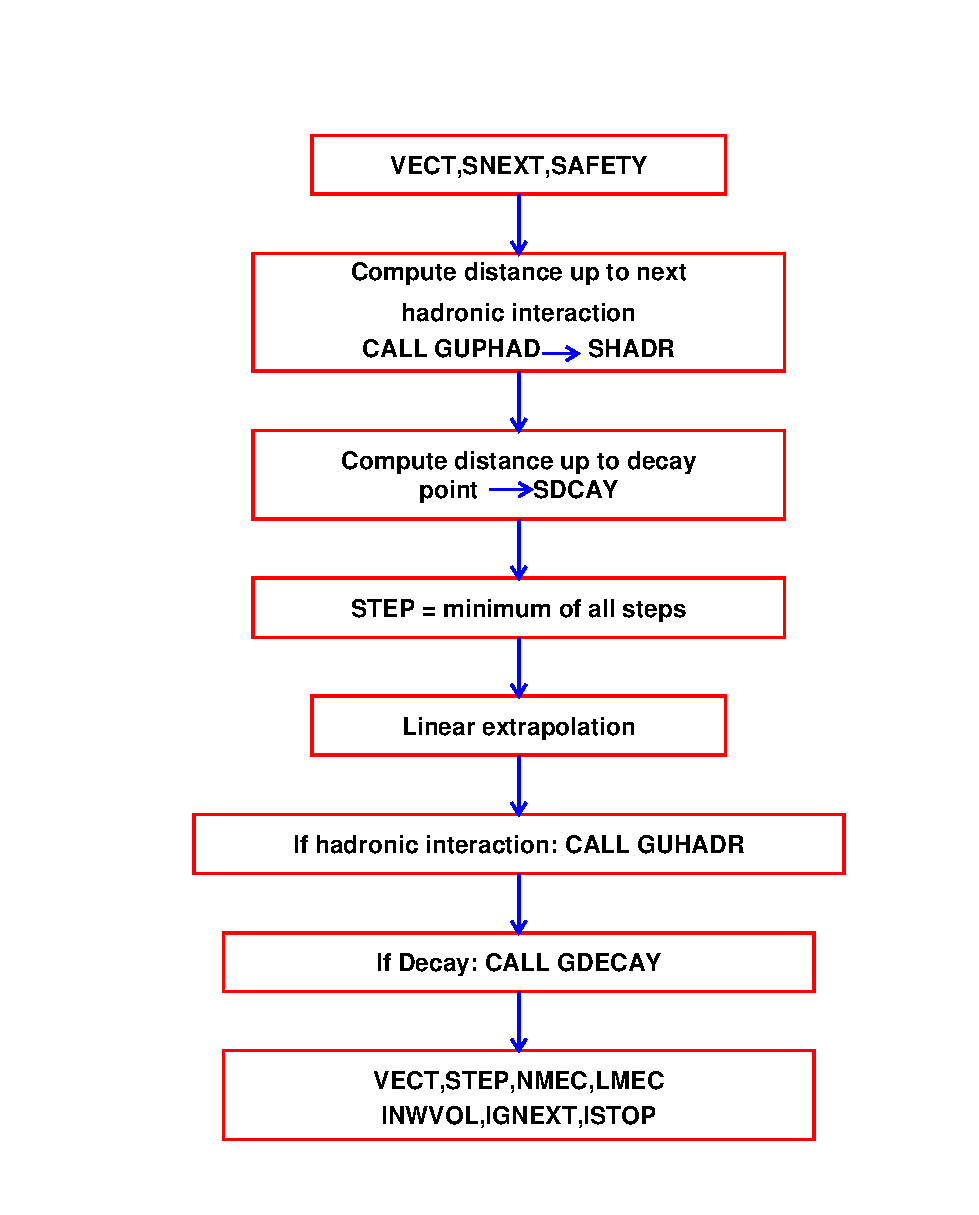
\epsfig{file=eps/trak200-4.eps,width=14cm}
     \caption{{\tt GTNEUT} block diagram}
     \label{fg:trak200-4}
\end{figure}

\begin{figure}[hbt]
     \centering
     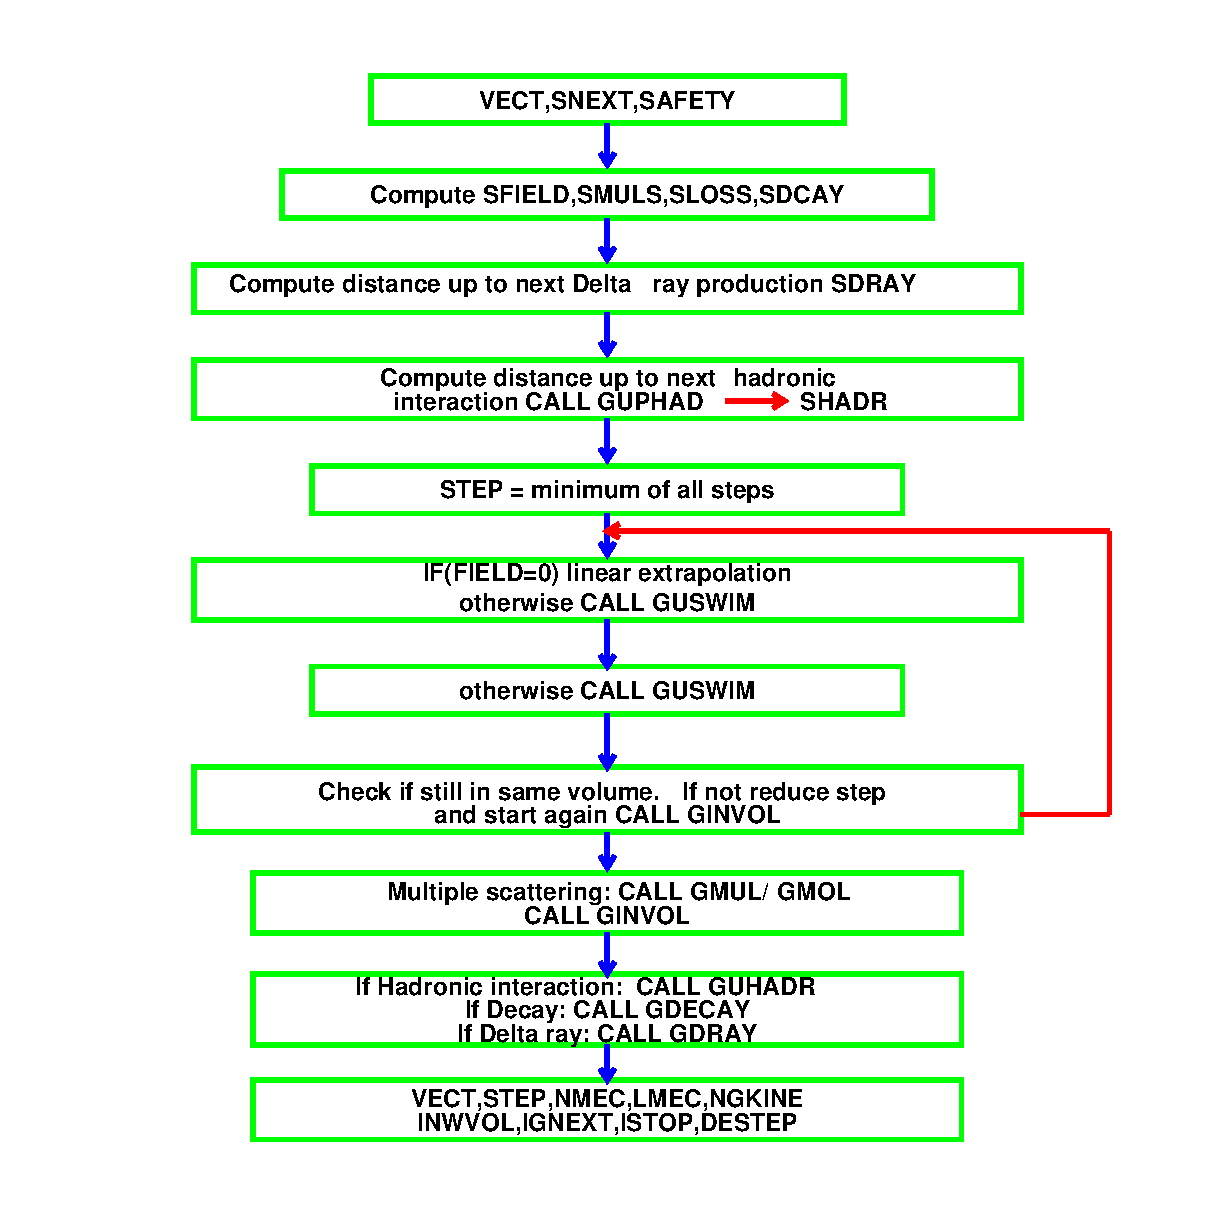
\epsfig{file=eps/trak200-5.eps,width=14cm}
     \caption{{\tt GTHADR} block diagram}
     \label{fg:trak200-5}
\end{figure}

\begin{figure}[hbt]
     \centering
     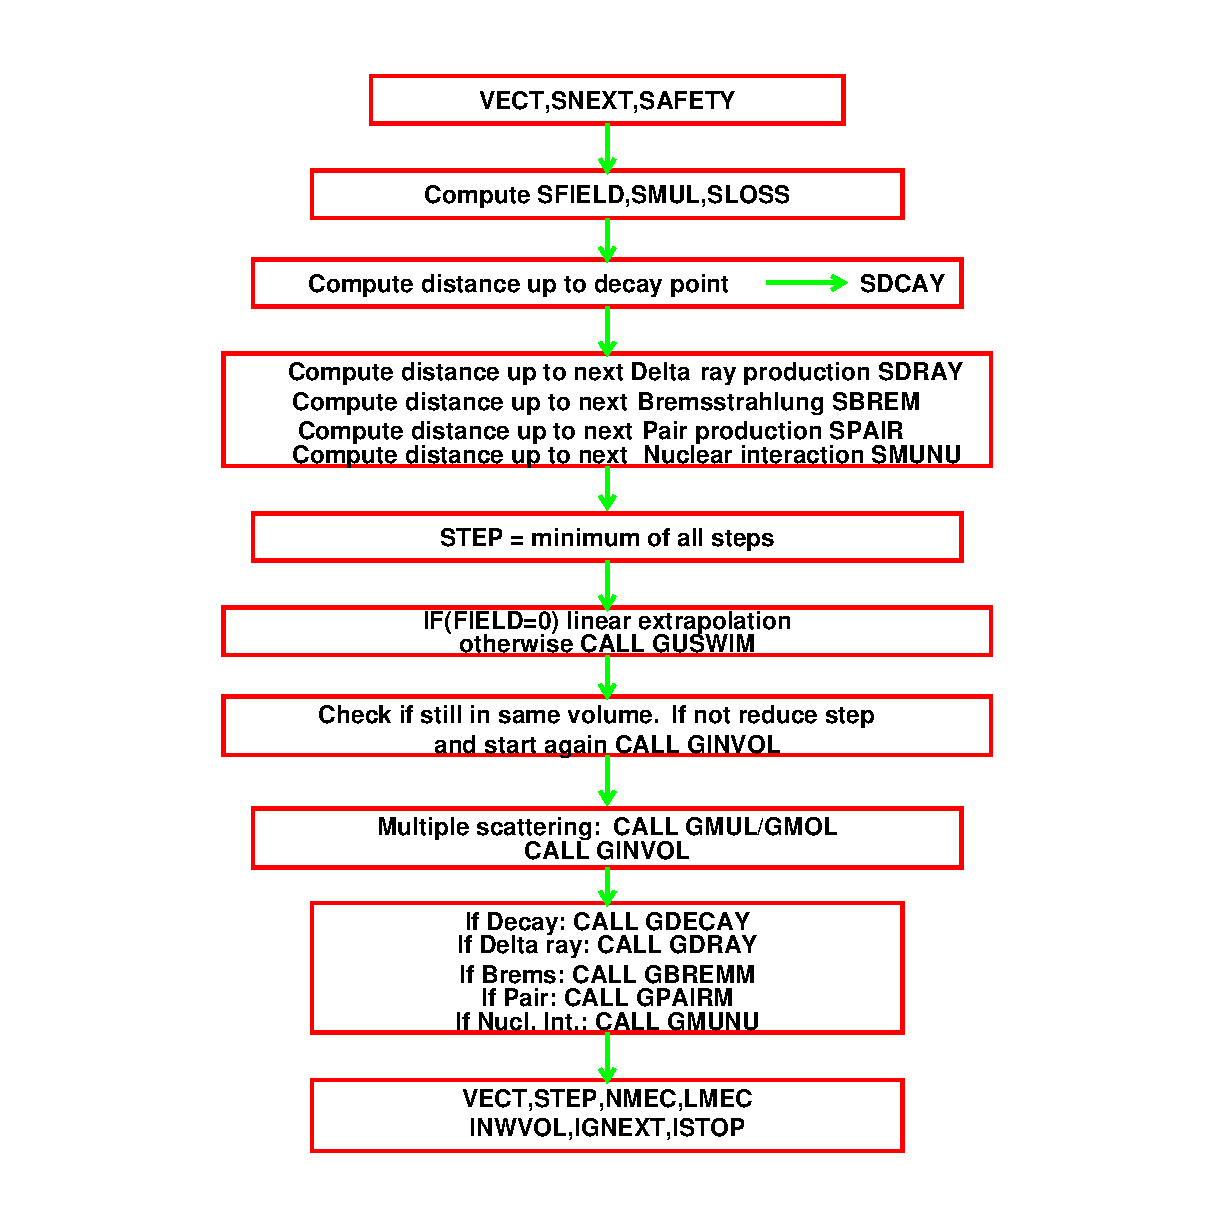
\epsfig{file=eps/trak200-6.eps,width=14cm}
     \caption{{\tt GTMUON} block diagram}
     \label{fg:trak200-6}
\end{figure}
%
%\begin{figure}[hbt]
%     \centering
%     
\epsfig{file=eps/trak200-7.eps,width=14cm}
%     \caption{{\tt GTNINO} block diagram}
%     \label{fg:trak200-7}
%\end{figure}
%
%\begin{figure}[hbt]
%     \centering
%     
\epsfig{file=eps/trak200-8.eps,width=14cm}
%     \caption{{\tt GTCKOV} block diagram}
%     \label{fg:trak200-8}
%\end{figure}
%
%\begin{figure}[hbt]
%     \centering
%     
\epsfig{file=eps/trak200-9.eps,width=14cm}
%     \caption{{\tt GTHION} block diagram}
%     \label{fg:trak200-9}
%\end{figure}

